
\begin{wrapfigure}{r}{10cm}
  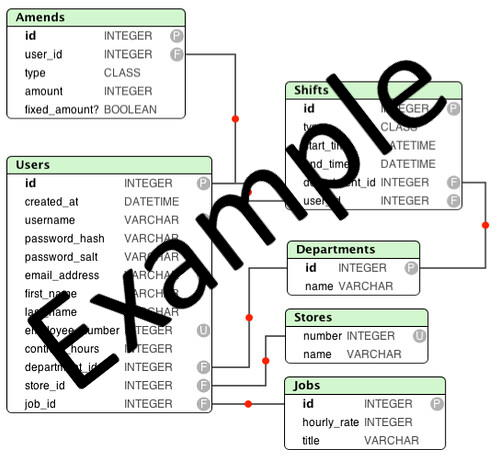
\includegraphics[width=\linewidth]{img/example_erd1.jpg}
  \caption{Entities and their relationship in the data}
  \label{fig:entity-relationship-diagram}
\end{wrapfigure}

The section discusses two distinct data needs. What is used for research and what is used in the interventions. The data for research is denominalized and seen by the research team, the data for the intervention is nominalized and only seen by the physician who undertook the care of the patient mentioned.

Patient and physician data will come from an existing system at the MUHC called the "data warehouse" (DW). A data warehouse is an enterprise data aggregation system which facilitates its collection, analysis, and reporting. The MUHC DW is already in place and contains a wide range of data relating to most aspects of in-hospital care.

This project will use two datasets coming from the same source. A first, broader and denominalized, data request will be made for the purpose of finding targets in objective one and two. This request will be placed to the research pipeline of the data warehouse. Here, the identity of both the patient or provider is of little interest as long as they have unique IDs. A second, precise, targeted, and nominalized data request will be made for the purpose of conducting the RCT. During this phase, I need to be able to have the right provider see the right feedback, but these providers also need to be able to see which patient might be in need of additional actions.

Additional data will be collected on the physician's use of e-A\&F. This data will be linked to anonymous IDs.

All nominalized data will be kept in a remote secure server in the MUHC data center. Feedback will also be created by the systems on this server. Anonymous data will be kept on a secure password protected computer, where the data analysis will also take place. All nominalized data will be removed as soon as the trial is over, while summary description of the anonymous data will be published along with the relevant research articles.